\item A disc of mass \( m = 50 \) g slides with the zero initial velocity down an inclined plane set at an angle \( \alpha = 30^\circ \) to the horizontal; having traversed the distance \( l = 50 \) cm along the horizontal plane, the disc stops. Find the work performed by the friction forces over the whole distance, assuming the friction coefficient \( k = 0.15 \) for both inclined and horizontal planes.
    \begin{center}
        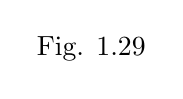
\begin{tikzpicture}
            \node at (0, 0) {Fig. 1.29};
        \end{tikzpicture}
    \end{center}\begin{solution}
    \begin{center}
        \begin{tikzpicture}
            \pic at (0, 0) {frame=3cm};
        \end{tikzpicture}
    \end{center}

    \begin{align*}
        \intertext{Let \(s\) be the distance covered by the disk along the incline, from the equation of increment of mechanical energy of the disk in the field of gravity: \(\Delta T + \Delta U - A_{fr}\)}
        0 + (-mgs\sin\alpha) &= -kmg\cos\alpha \cdot s - kmgl\\
        \intertext{or}
        s &= \dfrac{kl}{\sin\alpha - k\cos\alpha} \tag{1}
        \intertext{Hence the sought work}
        A_{fr} &= -kmg[s \cos\alpha + l]\\
        A_{fr} &= -\dfrac{klmg}{1 - k \cos\alpha} \quad \text{(using Eq. 1)}
        \intertext{On putting the values}
        A_{fr} &= -0.05 \, \text{J}
    \end{align*}
\end{solution}